\chapter{Large Scale Mining in Software Heritage}

As the field of software mining is constantly growing, notably for the purposes
of assessing and understanding the dynamic evolution of software projects,
there is a clear interest on the part of \gls{ESE} researchers and industrials
in accessing the data stored in the Software Heritage archive.

The main direction of the work presented in this thesis is to make large-scale
analysis of this immense body of data possible in an efficient manner. We limit
our scope to the software artifacts themselves, as studying external project
management metadata (issues, \acrshort{CI}, mailing list discussions, etc.) is
a largely different problem, although relevant to the field in its own way.

For that purpose, we first catalogued different use-cases by looking at
software mining studies and qualitatively assessing which types of data they
were extracting for their own purposes. This gives us a general idea of the
general queries researchers would want to run on the archive given the
opportunity to do so.

Of course, we cannot restrain ourselves to use cases we find in the literature,
as the scopes of past studies are endogenous to the infrastructure researchers
had at their disposal while conducting it. Part of our goal in making Software
Heritage a platform for universal software mining is to make new research
opportunities available by allowing researchers to run studies that were not
possible before. Therefore, in addition to the use cases we find in the
literature, we also want to understand general interests for future research
directions as a way to expand this horizon of possibilities.

\vspace{0.5cm}

This chapter is based on an article~\cite{swh-benevol2018-universal-analysis}
accepted at the 17th Belgium-Netherlands Software Evolution Workshop (BENEVOL
2018).

\section{Cataloguing Research Needs}

\subsection{Literature Review}

Being familiar with the software mining literature, and after various
preliminary conversations with researchers working in the field, we have
preconceived notions of how they design studies on software repositories. We
know the process is generally two-fold. The first step is to precisely
\emph{select} the software artifacts that are relevant for the study using a
variety of criteria: studies on Java source code will select files ending with
the \texttt{.java} extension, studies on large projects will require a given
number of revisions in the project, etc. Once the artifacts have been selected,
researchers can \emph{analyze} this new corpus by running custom-made tools and
processing algorithms.

To validate this understanding of the literature more rigorously, we
systematically reviewed 54 papers published in the \emph{16th International
Conference on Mining Software Repositories (MSR 2019)}. In each paper, we were
looking for two important pieces of information: (1) what were the
\emph{selection criteria} used to narrow down the study to work on a specific
set of software artifacts, and (2) which types of \emph{analyzed data} are
required for their analyses.

\begin{figure}[b]
\begin{tikzpicture}[x=1pt,y=1pt,font=\tiny]
  \begin{sankeydiagram}[
    sankey tot length=90pt,%
    sankey tot quantity=54,%
    sankey min radius=15pt,%
    sankey fill/.style={%
      draw,line width=0pt,
      fill,
      lime!50,
    },
    sankey draw/.style={%
      draw=black,
      line width=1pt,
      line cap=round,
      line join=round,
    },
    %sankey debug,
    ]
    \sankeynodestart{54}{0}{p0}{0,100};

    \sankeyadvance{p0}{60pt}
    \sankeyfork{p0}{48/p1,6/ex1}
    \node[left=5pt of p0, align=center]
        {\footnotesize 54 papers\\ \footnotesize from MSR};

    \sankeyadvance{p1}{60pt}
    \sankeyfork{p1}{44/p2,4/ex2}
    \sankeyadvance{p2}{60pt}
    \sankeyfork{p2}{41/p3,3/ex3}
    \sankeyadvance{p3}{60pt}
    \sankeyfork{p3}{36/p4,5/ex4}
    \sankeyadvance{p4}{60pt}
    \sankeyfork{p4}{28/p5,8/ex5}


    {%
        \tikzset{%
            sankey fill/.append style={%
                line width=0pt,
                lime!50!green!50,
            }
        }
        \sankeyadvance{p5}{60pt}
        \sankeynodeend{28}{0}{p5}{p5}
        \node[right=15pt of p5, align=center]
            {\footnotesize 28 papers\\ \footnotesize reviewed};
    }

    {%
        \tikzset{%
            sankey fill/.append style={%
                line width=0pt,
                red!50!lime!50,
            }
        }
        \sankeyturn{ex1}{-90}
        \sankeyadvance{ex1}{20pt}
        \sankeynodeend{6}{270}{ex1}{ex1}
        \node[below=15pt of ex1, align=center]
            {6 papers:\\not mining\\software repos};

        \sankeyturn{ex2}{-90}
        \sankeyadvance{ex2}{20pt}
        \sankeynodeend{4}{270}{ex2}{ex2}
        \node[below=15pt of ex2, align=center]
            {4 papers:\\proprietary or\\homemade dataset};

        \sankeyturn{ex3}{-90}
        \sankeyadvance{ex3}{20pt}
        \sankeynodeend{3}{270}{ex3}{ex3}
        \node[below=15pt of ex3, align=center]
            {3 papers:\\no experimental\\methodology};

        \sankeyturn{ex4}{-90}
        \sankeyadvance{ex4}{20pt}
        \sankeynodeend{5}{270}{ex4}{ex4}
        \node[below=15pt of ex4, align=center]
            {5 papers:\\few handpicked\\projects only};

        \sankeyturn{ex5}{-90}
        \sankeyadvance{ex5}{20pt}
        \sankeynodeend{8}{270}{ex5}{ex5}
        \node[below=15pt of ex5, align=center]
            {8 papers:\\irrelevant\\methodology};
    }

  \end{sankeydiagram}
\end{tikzpicture}
\caption{Sankey diagram of the selection process in our literature review.}%
\label{fig:msr-review-sankey}
\end{figure}

Not all articles in our corpus were relevant to improve our understanding of
software mining studies and had to be removed from the review. In particular,
we excluded:

\begin{itemize}
    \setlength\itemsep{0em}
    \item 6 papers which were not actually mining software repositories (tool
        papers, polling study, meta-analyses, etc.);
    \item 4 papers which used software artifacts corpuses that cannot be
        reconstructed from a software archive (proprietary datasets,
        custom-built datasets, manual example generation, etc.);
    \item 3 papers where no experimental methodology was described;
    \item 5 papers which were analyzing a specific set of handpicked
        repositories, and in which the analysis was only relevant for these
        particular repositories;
    \item 8 papers which had an irrelevant methodology (demonstrations of tools
        for building software corpuses, extensive reliance on context such as
        code snippets from development chats or webpages, etc.).
\end{itemize}

In total, we removed 26 papers as shown in the Sankey diagram
in~\figref{fig:msr-review-sankey}, and included the 28 remaining papers in our
review.

\subsection{Selection criteria}

The review allowed us to confirm the common study pattern in two steps that we
identified: selection of a subset of artifacts on some criteria, then analysis
of the selected artifacts. Table~\ref{tab:selection-criteria} shows a detailed
tally of the different criteria we observed in the study designs.

\begin{table}
    \begin{tabular}{l l c}
        & \textbf{Criteria} & \textbf{Number of studies} \\
         a. & Number of repository stars & 12 \\
         b. & Programming language of repository & 10 \\
         c. & Matching string or pattern in file contents & 5 \\
         d. & Pre-established list of URLs & 4 \\
         e. & File names and extensions & 4 \\
         f. & Natural language used in the project & 2 \\
         g. & Number of commits or releases & 2 \\
         h. & Number of forks & 2 \\
         i. & Random sampling & 2 \\
         j. & Commit dates & 1 \\
         k. & Licenses & 1 \\
         l. & Number of issues or pull-requests & 1 \\
         m. & Number of contributors & 1 \\
         n. & File sizes & 1 \\
         o. & Lines of code in contents & 1 \\
    \end{tabular}
    \centering
    \caption{Selection criteria found in MSR literature review.}%
    \label{tab:selection-criteria}
\end{table}

While some of these criteria would be easy to implement in the archive as a way
to select a subset of artifacts for a given study design, others would require
more work. They can be categorized in several groups, ordered by difficulty of
implementation:

\begin{itemize}
    \setlength\itemsep{0em}
\item \emph{Direct Addressing} (crit.\ d): when the study methodology includes
    a pre-established list of artifact identifiers (e.g., repository URLs or
    revision hashes). As long as a mapping between the unique identifiers and
    the objects in the graph is properly maintained, selecting objects based on
    their identifiers should be trivial.

\item \emph{Artifact Properties} (crit.\ e, g, j, n, m): selection is
    often done on properties that are directly stored as part of the artifacts
    themselves, like commit authors or dates, file names etc. This data is
    already present in the database and should only require indexes that allow
    to return all objects matching a given property, assuming these indexes
    were performant enough.

\item \emph{External Metadata} (crit.\ a, l): when the selection uses
    metadata that is not part of the software data tracked in the archive
    itself (contextual popularity information such as number of GitHub stars or
    pull requests). While external metadata is out of scope for this thesis, we
    should acknowledge the frequent need for researchers to filter on
    external and contextual metrics, and leave open the possibility of linking
    the objects in the archive with a metadata store.

\item \emph{Derived Data} (crit.\ b, f, h, o, k): for filtering on properties
    that are not directly part of the data, but which can be derived from them.
    By running a programming language recognition tool on the file contents, we
    can index contents by their detected programming language and allow users
    to filter objects on this criterion. This requires additional indexes as
    well as processing pipelines to generate this derived data.  While some
    derived data can be easily generated (e.g., counting the lines of code in
    a file), the process can be more involved for others: filtering on the
    number of file changes introduced in a given commit requires computing the
    difference between the directory subtrees of all successive commit pairs.

\item \emph{Code Search} (crit.\ c): when the selection happens on the contents
    of the files themselves. Finding all the files containing a specific string
    or pattern is significantly harder than filtering on other artifacts
    properties. As we noted in Section~\ref{sec:swh-infrastructure}, the
    total size of the file contents is around two orders of magnitude larger
    than the rest of the database, which makes indexing a lot more demanding in
    terms of infrastructure requirements. In addition, the problem of full-text
    search in source code is a notably hard one, as it requires a high level of
    expressiveness to be able to match on specific tokens or API uses.
\end{itemize}

Each selection criteria described here defines one specific filter on the
objects, but researchers generally combine these filters together to narrow
down their corpus of study. Therefore, it is not sufficient to simply provide a
way to select the data based on one of these filters; the partial filters must
be able to be joined together in a relational way to ensure enough
expressiveness in the selection phase.

\subsection{Analyzed Data}

After having selected the relevant objects of study using specific filters and
heuristics, researchers perform on them the analysis that constitutes the core
of their experimental design. In order to make this possible in Software
Heritage, it is necessary to understand which categories of data need to be
made accessible.

\begin{table}
    \begin{tabular}{l l c}
        & \textbf{Data type} & \textbf{Number of studies} \\
         a. & File contents & 15 \\
         b. & File names & 10 \\
         c. & Commit graph and commit properties & 9 \\
         d. & Commit diffs & 7 \\
         e. & Authors and community graph & 5 \\
         f. & Dependency data & 2 \\
    \end{tabular}
    \centering
    \caption{Types of analyzed data found in MSR literature review.}%
    \label{tab:analyzed-data}
\end{table}

In the MSR review, we identified 6 categories of data that were
frequently analyzed in mining studies, shown in Table~\ref{tab:analyzed-data}.

By far the most common type of analyzed artifacts is contents, highlighting the
clear need to make the source code files easily accessible. While there are
some studies which only rely on the upper layers of the artifact graph like
community detection algorithms, research on the source files themselves is
evidently of foremost interest for software mining.

Studies generally also require basic artifact properties like file names,
commit messages, dates and authors, etc. Those fields should be relatively easy
to provide from the Merkle DAG of the archive. Some studies also depend on the
topology of the subgraphs themselves: commit chains when analyzing software
evolution, subtrees when looking at file hierarchies. This is important to keep
in mind, as it means we cannot always simply provide an unorganized flat stream
of artifacts, and need to leave open the possibility of running algorithms on
the graph which links them together.

Here again, studies will tend to use derived data which can be computed from
the data in the archive. The most prominent example is commit diffs, as a lot
of studies look at the \emph{changes} that were introduced by each commit.

Some types of derived data can pose additional challenges. For instance,
computing dependency graphs will involve a different process for each
programming language, or even each package manager. For complex cases such as
this one, our focus should be to make sure all the objects required to compute
the derived data can be provided, so that researchers can generate the corpus
themselves.

\section{Functional requirements}

While a literature review gives us a good understanding of how \emph{current}
software mining studies are designed and the main categories of data they
exploit, they should not necessarily be our sole guide for the capabilities we
want to provide in a research platform. While the current literature reflect
the state of what is currently achievable for researchers, one of our goals is
to open-up new possibilities by leveraging the unique properties of the
archive, notably its canonical format, diversity and universality.

To that end, the efforts in building a mining platform in Software Heritage
should primarily focus on capabilities that would be uniquely impactful on the
state of the art when applied to this particular software development corpus.
Mining studies on handcrafted datasets, small number of repositories or
using metadata more easily accessible in other platforms (e.g., dependency
graphs, call graphs), while important to the field, might not be the most
suited for Software Heritage, at least in its first iterations. As a general
rule of thumb, a major strength of running experiments on the archive is that
the universality of the corpus can allow researchers to analyze public source
code exhaustively. This benefit is mostly present when the processing step can
largely be automated; studies requiring a lot of manual curating can leverage
the archive only to a minor extent and will not be our main focus.

As an initial target for the research platform, we identified five main
categories of research requirements for capabilities that we want the platform
to have:

\textbf{Content access}. One of the most common requests is to obtain a set of
file contents stored in the archive based on some specific criteria. Those
requests are usually made in the purpose of analysing the code itself: code
patterns recognition, language detection, static analysis, malware detection,
and so on.  Occasionally, those requests also require some data preprocessing
to be applied to the file contents before the analysis (comments removal, data
or binary strings removal, etc.).

\textbf{Filtering on metadata}. It is generally useful to filter the query
results depending on some criteria on the metadata of the files. This metadata
can be either already present in the archived repositories (file extensions,
file names, file sizes, directory depth…), or derived from the data (MIME
types, detected programming language, license…). This metadata has to be
precomputed and indexed along with the files.

\textbf{Content search}. The ability to perform full-text search for
specific code fragments or patterns is very useful to focus
computations on the relevant parts of the code, and it requires an up
to date full-text search index.

\textbf{History graph}: The ability to access the revision history graph along
with its associated metadata (authors, commit messages, etc.) and being able to
examine the relationships between the different objects in the revision graphs
is imperative to analyze not only the software itself but its evolution through
time. In the context of Software Heritage, these relationships also express
themselves across different repositories: forks point to the same ancestor
nodes, directories that were moved from one repository to another point to the
same object, etc.

\textbf{Provenance indexing}: While the software DAG works top-down (the nodes
only point to their children i.e., their content, but never their parents), it
is also sometimes necessary to be able to list the different parents that point
to a specific object. There are multiple applications for this: find the
possible extensions of a file, the different repositories that contain a code
fragment, a directory or a revision, etc. These traversals on the transposed
version of the DAG are known as ``provenance'' queries, as they allow us to
find out the sources of specific objects.

Of course, the platform should be flexible enough for complex queries that
combine multiple of these capabilities together. For instance, it should be
possible to find all contents referenced from a file with a specific extension
and which contain some specific function name, or to search nodes in the
history graph of a repository while filtering on their associated metadata.

\section{Challenges}

\subsection{Data volume}

Most of the challenges which stand in the way of providing some form of access
to the data directly stem from the sheer size of the software archive. Allowing
people to locally retrieve a large chunk of the archive to perform local
computations is very impractical at the Software Heritage scale in most cases,
both from a network transfer perspective and for the undue burden it would
cause on local storage requirements.

Handling the file contents of the archive requires a lot of resources and
expertise. The total size of the blobs (currently $\approx 700$ TB) require
a lot of storage capacity, and the blobs cannot easily be stored on a single
machine using consumer-grade storage. The unusual size distribution of the
blobs, whose median size is approximately 3~kB, makes it also hard to use
industry-grade storage solutions, because they often are not designed to store
a large quantity of very small files. On conventional systems, some limitations
on inode management may apply. Other distributed storage solutions like Ceph
cannot easily handle a large amount of small files (because of the per-file
overhead needed for replication~\cite{dandrimont2018cephml}), and require some
form of custom content packing to take place beforehand.

Compressing the blobs works well to reduce the size with a compression
ratio of $\approx 2$ (estimated on a random sample of about 1\% of the
archive). Further techniques based on ``packing heuristics'' to compress
similar contents together should be investigated to reduce their size even
more.

The size of the Merkle DAG itself is more reasonable (around 6 TB when stored
in the relational database format), but using it efficiently often requires
various indexes, which significantly increases its size on-disk.  Moreover,
some intensive processing on the graph itself could require having it stored
directly in main memory, which is difficult to achieve on standard machines
that have orders of magnitude less RAM.\@

Even if the recipient of the dataset already has the storage capacity and
expertise to handle such a vast amount of data, transferring it through the
network is impractical and expensive. Sending the whole dataset through a
connection with a speed matching the common industry standard of 1~Gbps would
take more than 60 days, assuming the absence of sequential overhead between
fetches.

\subsection{Representation mismatch}

Researchers and data scientists usually try their experiments by prototyping on
small sample sizes, before reaching out to experiment on larger datasets.
Doing so, they generally use tools that are fit for specific data
representations, and thus they often expect the data to be presented in
specific formats. One of the challenges of making software analysis accessible
to them is to help them transform the data from a format well-suited for
\emph{archival} to a format suited for large-scale \emph{analysis}.

Files and directories contained in a specific revision are usually expected to
be represented as on-disk filesystem trees, so the children of the
directories can directly be accessed through the primitives of the filesystem.
In the Software Heritage archive, the de-duplication requires this to go
through an additional index of the hashes of the directories. The interface
therefore has to provide a utility to ``flatten'' the compact representation
into a more classical directory structure, although doing so systematically
would invalidate the benefits of de-duplication.

For the revision graph itself, there is no current standard of representation,
so most of the research experiments so far have worked on tool-specific
representations (often depending on the version control system used). While
there is value in providing a universal representation for commit-level
software evolution from different sources, it is still important to provide a
data representation that does not stray too far from what those domain-specific
analysis tools usually expect.

\subsection{Provenance mappings}

Making provenance mappings accessible as a way to look up the different
places where an object can be found is a hard problem, because of the
combinatorial explosion of the ancestor relationship mappings.
A single file content can be found in thousand if not millions of origins.
There is a difficult balance to find between reducing the size of the
mappings using intermediate objects in the relationship as layers to compress
the volume of edges, and reducing as much as possible the amount of
indirections that require index hits for performance reasons.

Moreover, maintaining this (bottom-up) provenance index is harder than its
top-down counterparts, since there is no way to know in advance all the objects
of the relationship, and thus represent them with an intrinsic hash for
indexing. These mappings will therefore have to be dynamic, meaning a
provenance query for a given software artifact will give different responses
as more snapshots get archived.

\subsection{Repeatability and reproducibility}

An important part of scientific experiments is reproducibility, which is
something to keep in mind when making a very large and
constantly-evolving dataset available for research applications. While
intrinsic hashes guarantee full consistency of the data at the snapshot level,
it might be useful to provide a way to describe the state of the \emph{entire
  archive} at some point in time. If we are able to reconstruct a previous
state of the archive from a timestamp, including this timestamp along
with the experiment methodology will allow the experiment to be repeated on the
exact same dataset as when it was performed for the first time. That way, an
experiment can be \emph{repeated} by performing it on the timestamped state of
the archive, and \emph{reproduced} by performing it on a different dataset.

The naive way to get an intrinsic identifier a Merkle DAG is simply to hash the
list of roots, however it does not work when the graph is incomplete. As the
Software Heritage DAG can have a lot of holes (missing revisions, files, etc.)
that can be added or removed without changing the intrinsic identifier of the
nodes, relying solely on those hashes is not sufficient to reliably get a
hash of the archive as a whole.

A better way to achieve this would be to use the journal described in
Section~\ref{sec:swh-infrastructure} by adding timestamps to each inserted
objects, then read all the objects from the journal up to the archive timestamp.

\subsection{Expressiveness}

Researchers who want to run analyses on the Software Heritage dataset will
perform \emph{queries} on the archive to describe the computations and the part
of the archive they will be run on. Running these queries on the archive will
require a query API that can express these different use cases.

The expressive power of the query language determines how easy it is to use
the different data selection features, computation primitives and result
aggregations when running queries on the dataset. The semantics of the language
have to provide ways of representing and combining those different operations
so that the breadth of computations that queries are able to represent is as
wide and generic as possible for the use-cases we identified.

\section{Roadmap}

\begin{figure}
\begin{center}
    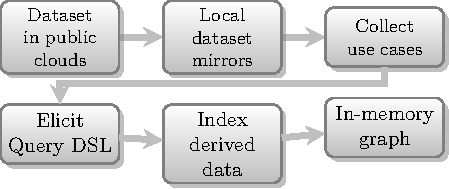
\includegraphics[width=0.55\textwidth]{img/roadmap}
\end{center}
\caption{Steps towards creating a research platform in Software Heritage}%
\label{fig:roadmap}
\end{figure}

A preliminary step of this work is to make the dataset available in some
format suitable for scale-out analysis, so that Software Heritage and other
researchers can try out a few experiments and document their own use-cases.
Some public cloud computing providers like Amazon Web Services or Google Cloud
have public datasets programs, on which we can make the Software Heritage
dataset publicly available without bearing the cost of the storage.

While allowing people to run queries directly on a public cloud instance is
well-suited for one-off experiments, it does not always work well for more intensive
use-cases. Researchers having access to hardware resources and software engineering
skills might find it more cost-efficient to run their experiments on a local
copy of the archive. As we build a pipeline to keep the Software Heritage
public datasets up to date, we need to provide a way for researchers to have
their own local copy of the dataset for in-house processing.

Once the dataset is available in some format for people to run queries on it,
we will be able to collect more real-world use-cases as a way to improve our
understanding of researchers' needs, which in turn guides the platform design:
what are the types of queries that scientists want to run? What are the data
and metadata filters that they need?  What is the kind of information that is
the most often retrieved from the data model?

After having collected these use-cases, it is then be possible to elicit a
domain specific language that can cover the kind of queries required
for the use-cases we identified, to offer a more accessible interface than
doing raw queries on the database. This language will have to be expressive
enough to address the difficulties we outlined, notably by allowing flexible
manipulations of the data representations. It should also be as simple as
possible to express constraints on the data used for the computations, and to
limit the span of the queries.

Real-world use cases also exhibit patterns of access to data derived from
the dataset, like diffs between revisions, branching and merging histories,
etc. Isolating this ``derived data'' to index it in the dataset would also be
useful to the platform, as it would significantly improve the performance of
computations on these common use cases.

While the cost of disk access for the file contents cannot be avoided, another
interesting research direction performance-wise will be to store as much of the
history graph as possible directly in memory. This should allow for efficiently
query the complex structures that constitute the archive graph and allow us to
analyze it in more detail.
